
\documentclass[letterpaper, 10 pt, conference]{ieeeconf}  
\IEEEoverridecommandlockouts                             
\usepackage{graphicx} 
\usepackage{hyperref}

\overrideIEEEmargins

\title{\Huge Dense Optic Flow}
\author{Jiyu Tian} 

\begin{document}

\maketitle
\thispagestyle{empty}
\pagestyle{empty}

%-------------------------------------------------------------------------

\section{INTRODUCTION}
In this project we explore the implementation of the Lucas-Kanade method for estimating dense optic flow from a pair of images. We take a pair of greyscale images taken from a video sequence as the input, and output two matrices containing the x and y components of the flow vector at each pixel.
%-------------------------------------------------------------------------
\section{ALGORITHMS DESCRIPTION}


\subsection{Grayscale Conversion}
After reading in two images, we first make them grayscale. We apply the conversion as the following equation:
\begin{equation}
Gray = 0.299 \times R + 0.587 \times G + 0.114 \times B
\end{equation}

If, in the worst case, input images do not have all the three $RGB$ channels, we simply regard the first channel as its grayscale value.



\subsection{Image Gradient}
Before taking the derivative, we smooth the images using Gaussian filter. The spatial intensity gradients $I_x$ and $I_y$ of second image is computed using horizontal and vertical components of Prewitt/Sobel mask. Compute the temporal gradient $I_t$ by subtracting a smoothed version of first image from a smoothed version of the second image.


\subsection{Lucas-Kanade Method}
For a given $N\times N$ window, a system of linear equations can be formed at each pixel by summing over products of gradients in its neighborhood. That is, at each pixel, we have a set of equations:
\begin{equation}
\left[ \begin{array}{cc}
\sum I^2_x & \sum I_xI_y\\
\sum I_xI_y & \sum I^2_y
\end{array} \right] \left[ \begin{array}{c}
V_x\\
V_y
\end{array} \right]= -\left[ \begin{array}{c}
\sum I_xI_t\\
\sum I_yI_t
\end{array} \right]
\end{equation}

The flow vector $[V_x, \ V_y]$ can then be solved at each pixel. $[V_x, \ V_y]$ will be $[0, \ 0]$ if the left matrix do not have full rank.


\subsection{Scaling}
One main assumption for LK method is that the motion is small. If the motion is large and violates this assumption, we need first reduce the resolution of images and then apply the Lucas-Kanade method.
%-------------------------------------------------------------------------
\section{EXPERIMENTAL RESULTS}
Before applying LK method, the input images are converted into grayscale, and smoothed by $7\times7$ Gaussian filter with $\sigma = 1.4$.
\begin{figure}[thpb]
\centering
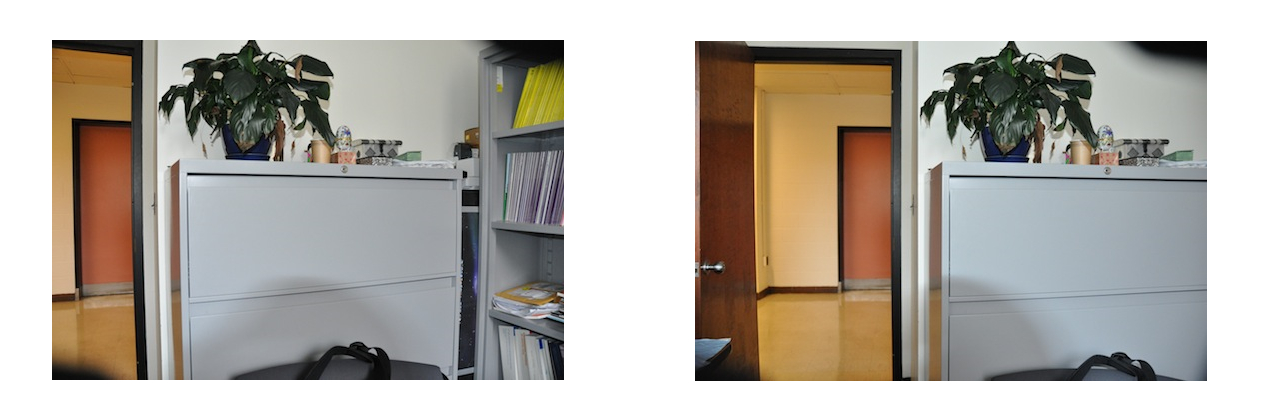
\includegraphics[width=0.4\textwidth]{raw.png}
\caption{Raw Images}
\label{mosaic}
\end{figure}

\subsection{Scale}

\begin{figure}[thpb]
\centering
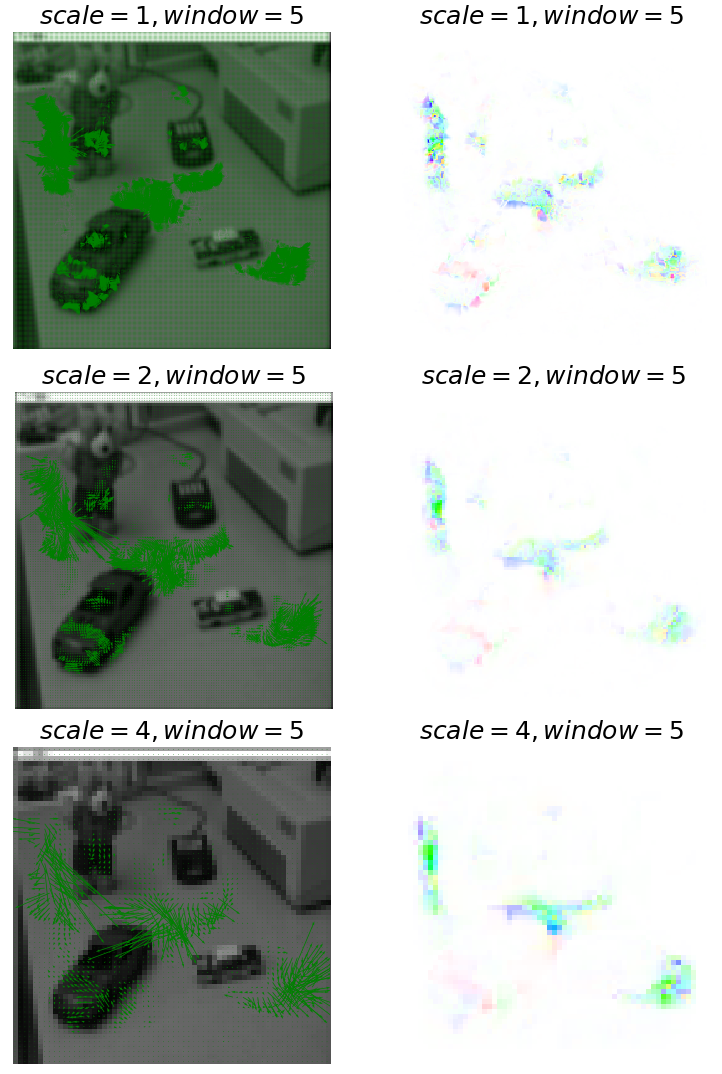
\includegraphics[width=0.42\textwidth]{scale5.png}
\caption{Different Scale}
\label{scale}
\end{figure}

\clearpage

\begin{figure}[thpb]
\centering
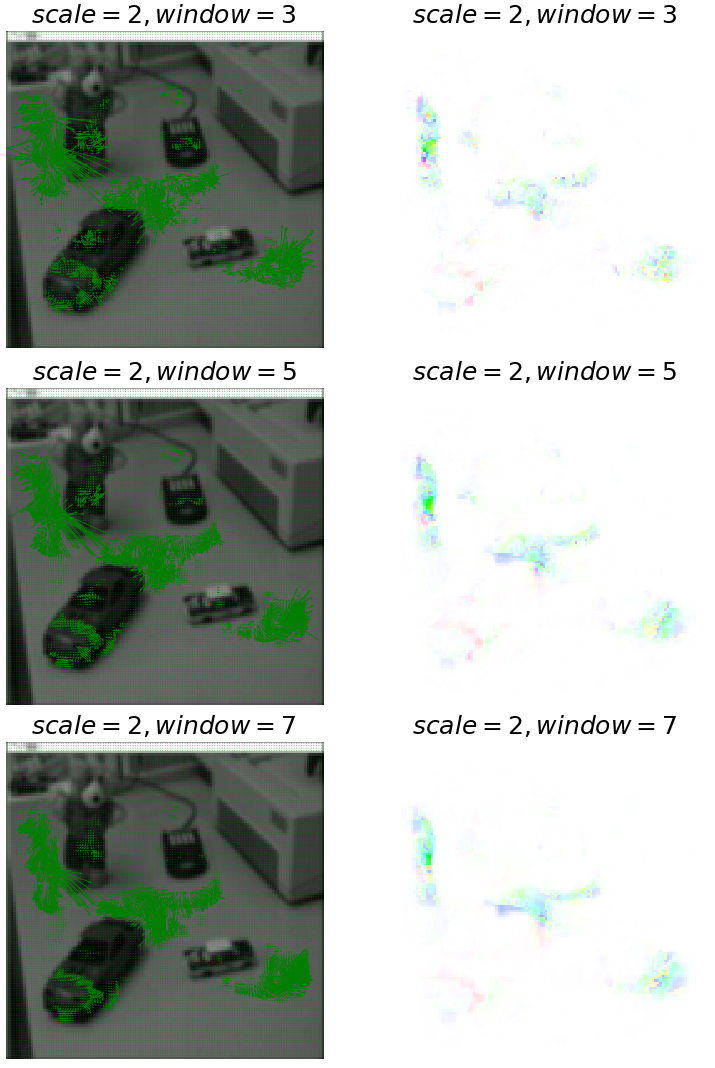
\includegraphics[width=0.4\textwidth]{window2.png}
\caption{Different Size}
\label{window}
\end{figure}



As we down-sampling the image, the pixel spacing is also reduced. We can see from Figure \ref{scale} that the optical flow tends to be uniform, and the algorithm is performing better. But still we notice that there are several vectors with extreme large magnitude.



\subsection{Window Size}
As we can see from Figure \ref{window}, larger window size also results in better performance given a fixed scaling factor. 
\newpage
The window size must be large enough to have sufficient intensity variation for detection, yet a too large one may contain pixels with different disparity.



\subsection{Limitation}
One big limitation of Lucas-Kanade method is that it may fail on large motion. Although this can be slightly modified by reducing image resolution, yet poor resolution can also be a great problem for the method.

Also as we can see from Figure \ref{limit}, the method also highly depends on brightness constancy and camera calibration.

\begin{figure}[thpb]
\centering
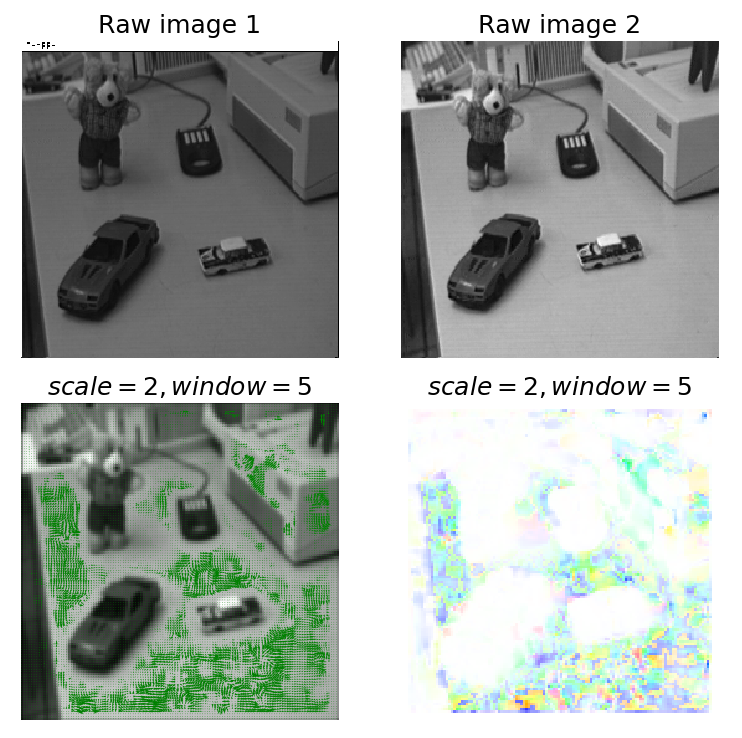
\includegraphics[width=0.415\textwidth]{limit.png}
\caption{Limitation}
\label{limit}
\end{figure}
%-------------------------------------------------------------------------
\section{CONCLUSION}
In this project, we implemented Lucas-Kanade method for optical flow estimation. We also explored influence from various parameters, as well as the limitation of the method.
\vfill

\end{document}
